\documentclass[abstracton,12pt]{scrreprt}

\usepackage[utf8]{inputenc}
\usepackage[T1]{fontenc}
\usepackage{fancyhdr}
\usepackage{graphicx}
\usepackage{tikz}
\usepackage{times}
\usepackage{listings}
\usepackage{amssymb}
\usepackage{amsfonts}
\usepackage{amsmath}
\usepackage{algorithm}
\usepackage{algpseudocode}




% --------- 

\titlehead{Department of Informatics, University of Zürich}
\subject{\vspace*{2cm}BSc Thesis}
\title{Implementing an Index Structure for Streaming Time Series Data}
\author{
  Melina Mast\\[-5pt]
  \scriptsize Matrikelnummer: 13-762-588\\[-5pt]
  \scriptsize Email: \texttt{melina.mast@uzh.ch}
}
\date{\vspace*{2cm}August, 2016}
\publishers{
  \small supervised by Prof.\ Dr.\ Michael Böhlen and Kevin Wellenzohn \\[5cm]
  \begin{tikzpicture}[overlay]
    \node at (-3,-3) {
\includegraphics[height=5.5cm]{IFIlogo}};
    \node at (7,-3) {
\includegraphics[height=2cm]{dbtgBW}};
  \end{tikzpicture}
}

%----\dedication{dedicated to xxx}

% --------- 

\newtheorem{definition}{Definition}
\newtheorem{example}{Example}
\newtheorem{theorem}{Theorem}
\newtheorem{lemma}{Lemma}

\newenvironment{proof}
  {\noindent{\bf Proof:\rm}}{\hfill$\Box$\vspace{\medskipamount}}

\def\bbbr{{\rm I\!R}}
\def\bbbm{{\rm I\!M}}
\def\bbbn{{\rm I\!N}}
\def\bbbz{{\rm I\!Z}}

% --------- 

\begin{document}

\maketitle

\chapter*{Acknowledgements}

I especially would like to thank my supervisor Kevin Wellenzohn, who has supported me with guidance and constructive feedback during my work. Besides, I would like to thank Prof. Dr. Michael Böhlen for the opportunity to write my bachelor thesis at the Database Technology Group of the University of Zurich. ...   

\begin{abstract}
  ...
\end{abstract}

\chapter*{Zusammenfassung}

\tableofcontents
\listoffigures
\listoftables

\listofalgorithms


\chapter{Introduction}
The financial stock market, wireless sensor networks, weather forecasts or monitoring systems use streaming time series. A streaming time series is a unbounded sequence of data points that is continuously extended, potentially even forever.\\Since it is unbounded, a system cannot hold the constantly generated data in his main memory endlessly. Therefore, the data that is kept in main memory needs to be limited to a part of the time series. Besides, in order to be practical for a application like the financial stock market, the data that arrives in a defined time interval (e.g. every 2 minutes) needs to be completely processed until the succeeding data arises. 

\chapter{Background and Related Work}
\chapter{Problem Statement}
\section{Handling Duplicate Values}

B+ trees are often 

\subsection{Add the time to the key}
If you would add the timestamps to keys would be unique. So if the case occurs where you have the same keys but in different leaves because the leaves were full and had therefore be splitted you could include the timestamps which divides the two different values to the parent. --> every key with timestamp smaller than the parents timestamp is in the left leaf and every key with timestamp bigger or equal is in the right one --> 
Problems: more memory needed. always check needed if there is a timestamp in the leaf
+ neighbour method would still work because you have the value and the set of time stamps 

\subsection{Add several times to the key}

The second was to have just one entry for each key, but the 'payload' associated with each key points to a different block of data, which is a linked list pointing to all instances of items that are having the same key


\subsection{Not change insertion but the search algorithm}
There are several different ways of handling duplicate keys. One way is use an unmodified insert algorithm which allows duplicate keys in blocks but is otherwise unchanged. The issue with a structure such as this is the search algorithm must be modified to take into account several corner cases which arise
For instance one of the invariants of a B+Tree may be violated in this structure. Specifically if there are many duplicate keys, a copy of one of the keys may be in a non-leaf block. However, the key may appear in blocks that which appear logically before the block which is pointed at by the key in the internal block. Thus the search algorithm must be modified to look in the previous blocks to the one suggested by the unmodified search algorithm. This will slow down the common case for search.There is another issue with this straight forward implementation, if there are many duplicate keys in the index, the index size may be taller than necessary. Consider a situation were for each unique key there are perhaps hundreds of duplicates, the index size will be proportional to the total number of keys in the main file, however, you only need to index an index on the unique keys. One of the files indexed in our program will be indexing has such characteristics to its data. It indexes strings (as the keys) with associated instances where those strings show up in our documents. There can be hundreds to thousands of instances of each unique string.
Therefore the approach I took was to store only the unique keys in the index, and have the duplicates captured in overflow blocks in the main file. An example of such a tree can be seen in figure 2. Consider key 6; there are 5 instances of this key in the tree. The tree is order 3, indicating the keys cannot all fit in one block. To handle this situation an overflow block is chained to the block which is indexed by the tree structure. The overflow block then points to the next relevant block in the tree.To create a structure such as this, the insert algorithm had to be modified. Like the previous version these modifications do not come without a cost, in particular the invariant which states all block must be at least half full has been relaxed. This is not true in this B+Tree, some blocks like the one containing key number 7, are not half full. This problem could be partially solved by using key rotations to balance the tree better. However, there are still corner cases where there would be a block which is under-full. One such corner case includes when a key falls between two keys which have overflow blocks. It must then be in a block by itself, since this B+Tree has the invariant which state that if a block is overflowing it can only contain one unique key. In the future we would like to implement key rotations to help partially alleviate the problem of under-full blocks.

The advantage of this approach to B+Trees with duplicate keys is the index size is small no matter how the ratio of duplicate keys to the total number of keys in the file. This property allows our searches to be conducted quicker. Since the overflow blocks are chained into the B+Tree structure we still have the property of being able to fast sequential scans. One consequence is we have defined all queries on our B+Trees to be range queries. This is fine because all of our queries were already range queries. In conclusion we relax the condition that all blocks must be at least half full to gain higher performance during search.

http://hackthology.com/lessons-learned-while-implementing-a-btree.html

\chapter{Solution}




\chapter{Experimental Evaluation}

\section{Runtime Complexity}
\section{Space Complexity}

\chapter{Summary and Conclusion}

\section{Fixed-Period Problems: The Sublinear Case}

With this chapter, the preliminaries are over, and we begin the search
for periodic solutions to Hamiltonian systems. All this will be done
in the convex case; that is, we shall study the boundary-value problem
\begin{eqnarray*}
  \dot{x}&=&JH' (t,x)\\
  x(0) &=& x(T)
\end{eqnarray*}
with $H(t,\cdot)$ a convex function of $x$, going to $+\infty$ when
$\left\|x\right\| \to \infty$.

\begin{example} [{\rm(External forcing)}]
Consider the system:
\begin{equation}
  \dot{x} = JH' (x) + f(t)
\end{equation}
where the Hamiltonian $H$ is $\left(0,b_{\infty}\right)$-subquadratic,
and the forcing term is a distribution on the circle.
\end{example}

\subsection{Autonomous Systems}

We assume a \emph{time domain}, $\mathcal{A}$, as a set of time
instants equipped with a total order $\leq$ and isomorph to integers.
Time granularities are partitionings of subsets of $\mathcal{A}$ into
non-empty intervals of time instants, termed \emph{granules}.
Examples of time granularities are minutes ($\mathit{min}$), hours
($\mathit{hou}$), days ($\mathit{day}$), weeks ($\mathit{wee}$),
months ($\mathit{mth}$), and years ($\mathit{yea}$).  The granularity
$\mathit{day}$, for instance, divides the time domain into granules of
1440 minutes.  We assume a \emph{bottom granularity}, $G_\bot$, such
that each granule of $G_\bot$ contains exactly one time instant.  In
our running example minutes represent the bottom granularity, and we
use the ISO~8601:2004 notation to denote time instants, e.g.,
\mbox{2007-02-12 07:15}.  The granules of each granularity $G$ are
ordered according to the time domain order and indexed with a subset
of integers, $\mathcal{L}_G$, such that the indexing function
$\mathcal{M}_G : \mathcal{L}_G \to G$ is an isomorphism that preserves
the total order $\leq$. For each granularity we assume that the
granule with index~0 contains the time instant 2000-01-01-00:00.
Figure~\ref{fig:ch0-gran-labels} illustrates some correspondences of
indexes between different granularities, e.g.,
$\mathcal{M}_\mathit{day}(2599)$ = [2007-02-12 00:00, 2007-02-12
23:59].

For the conversion between different granularities, we adopt the
\emph{bigger-part-inside semantics}~\cite{Ohlbach06,ical98}.  The
conversion from a coarser granularity $H$ to a finer granularity $G$
is defined as
\begin{align*}
  \downharpoonright^{H}_{G}(i) = \{ j \mid
  & |\mathcal{M}_{G}(j) \cap
  \mathcal{M}_{H}(i)| > |\mathcal{M}_{G}(j) \setminus
  \mathcal{M}_{H}(i)| \lor {}
  \\
  & (|\mathcal{M}_{G}(j) \cap \mathcal{M}_{H}(i)| =
  |\mathcal{M}_{G}(j) \setminus \mathcal{M}_{H}(i)| \land
  \max(\mathcal{M}_{G}(j)) \in \mathcal{M}_{H}(i) )\}
\end{align*}
$\downharpoonright^{H}_{G}(i)$ returns the indexes of those granules
in $G$ that are covered by granule $i$ in $H$ for more than a half or,
if exactly half of a granule in $G$ is covered, the second half.

\section{Time Slices and Multislices}

A (time) \emph{slice}~\cite{Niezette92} is a finite list of pairs,
$\lambda = (G_1X_1,\ldots,G_dX_d)$, where $G_l$ are granularities and
$X_l$ are \emph{selectors} that are defined as sets of integers.  Each
selector $X_{l+1}$ specifies a set of granules in $G_{l+1}$ with a
relative positioning with respect to granularity $G_l$.  The sequence
of granularities $(G_1,\ldots,G_d)$ is the \emph{hierarchy} of the
slice.  

Consider the slice $(\mathit{yea}\{7\}, \mathit{wee}\{\text{0-25}\},
\mathit{day}\{\text{0-4}\}, \mathit{hou}\{7\},
\mathit{min}\{\text{0,25,55}\})$.  The hierarchy is $(\mathit{wee},
\mathit{day}, \mathit{hou}, \mathit{min})$.  The first selector
$\{7\}$ selects the year 2007, the selector \{0-25\} selects the first
26 weeks of this year, the selector \{0-4\} selects the days from
Monday to Friday from each of these weeks, etc.

The semantics of a slice $\lambda$ = $(G_1X_1$, \ldots, $G_dX_d)$ is
defined through the following mapping $\mathcal{I}$ to a subset of the
time domain:

\begin{equation*}
  \mathcal{I} (\lambda) =
  \begin{cases}
    \bigcup_{k \in X_1} \mathcal{M}_{G_1}(k) & d=1 \\[1ex]
    \mathcal{I} \left( (G_2\bigcup_{k \in X_1}(
      \downharpoonright^{G_1}_{G_2}(k)/^+X_2), \ldots, G_dX_d)
    \right) & d>1
  \end{cases}
\end{equation*}

Here, $\downharpoonright^{G_1}_{G_2}$ is a bigger-part-inside
conversion from a granularity $G_1$ to a granularity $G_2$, and
$\downharpoonright^{G_1}_{G_2}(k)/^+X_2$ is defined as
$\downharpoonright^{G_1}_{G_2}(k) \cap \{
\min(\downharpoonright^{G_1}_{G_2}(k)) + i \mid i \in X_2 \}$.

\begin{figure}[htbp]\centering
  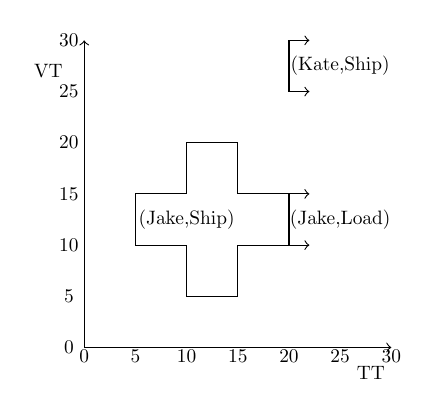
\begin{tikzpicture}[scale=0.13]
    \tikzstyle{every node}=[scale=0.7]
    \draw[->] (0,0) -- (30,0);
    \foreach \t in {0,5,10,15,20,25,30} \node at (\t,-0.9) {\t};
    \draw (28,-2.5) node {TT};
    \draw[->] (0,0) -- (0,30);
    \foreach \t in {0,5,10,15,20,25,30} \node at (-1.5,\t) {\t};
    \draw (-3.5,27) node {VT};
    \draw[<->] (22,10) -- (15,10) -- (15,5) -- (10,5) -- (10,10)
      -- (5,10) -- (5,15) -- (10,15) -- (10,20) -- (15,20) -- (15,15)
      -- (22,15);
    \draw (20,10) -- (20,15);
    \draw (10,12.5) node {(Jake,Ship)};
    \draw (25,12.5) node {(Jake,Load)};
    \draw[<->] (22,25) -- (20,25) -- (20,30) -- (22,30);
    \draw (25,27.5) node {(Kate,Ship)};
  \end{tikzpicture}
  \caption{Relationships between $P$, $M$, and $M_\mathrm{min}$}
  \label{fig:ch2-singular-minimal-mapping}
\end{figure}

\chapter{The Final One}

\begin{lemma}
Assume that $H$ is $C^{2}$ on $\bbbr^{2n} \setminus \{ 0\}$ and
that $H'' (x)$ is non-de\-gen\-er\-ate for any $x\ne 0$. Then any local
minimizer $\widetilde{qx}$ of $\psi$ has minimal period $T$.
\end{lemma}

\begin{proof}
We know that $\widetilde{x}$, or
$\widetilde{x} + \xi$ for some constant $\xi
\in \bbbr^{2n}$, is a $T$-periodic solution of the Hamiltonian system:
\begin{equation}
  \dot{x} = JH' (x)\ .
\end{equation}

There is no loss of generality in taking $\xi = 0$. So
$\psi (x) \ge \psi (\widetilde{x} )$
for all $\widetilde{x}$ in some neighbourhood of $x$ in
$W^{1,2} \left(\bbbr / T\bbbz ; \bbbr^{2n}\right)$.

But this index is precisely the index
$i_{T} (\widetilde{x} )$ of the $T$-periodic
solution $\widetilde{x}$ over the interval
$(0,T)$, as defined in Sect.~2.6. So
\begin{equation}
  i_{T} (\widetilde{x} ) = 0\ .
  \label{eq:five}
\end{equation}

Now if $\widetilde{x}$ has a lower period, $T/k$ say,
we would have, by Corollary 31:
\begin{equation}
  i_{T} (\widetilde{x} ) =
  i_{kT/k}(\widetilde{x} ) \ge
  ki_{T/k} (\widetilde{x} ) + k-1 \ge k-1 \ge 1\ .
\end{equation}

This would contradict (~\ref{eq:five}), and thus cannot happen.
\end{proof}

\begin{figure}[htbp]\centering

\end{figure}

A reference to a Figure~

\chapter*{Bibliography}

\bibliographystyle{alpha}
\bibliography{}

\end{document}
